% #region PREAMBEL OG PAKKER
\documentclass[a4paper, 12pt]{article}  % DOKUMENTKLASSE
\title{Øving 8}                         % TITTEL
\author{Håvard Solberg Nybøe}           % FORFATTER
\date{MA0301 -- \today}                 % DATO & FAG

\usepackage[english, norsk]{babel}      % NORSK SPRÅK
\usepackage[
    backend=biber,style=apa]{biblatex}  % BIBLIOGRAFI
\usepackage{csquotes}                   % PAKKE TIL BABEL
\addbibresource{bibliografi.bib}        % PATH TIL BIBLIOGRAFI
\usepackage[hidelinks]{hyperref}        % LENKER I TOC OG GENERELT
\usepackage[margin=1in]{geometry}       % VANLIG STØRRELSE MARGIN
\setlength{\parindent}{0em}             % SKILLER AVSNITT
\setlength{\parskip}{.8em}              % SKILLER AVSNITT
\usepackage{graphicx}                   % BILDER \includegraphics[OPTIONS]{PATH}
\usepackage{kantlipsum}                 % FYLLTEKST I KANT-STIL (kant[n-m])
\usepackage{amsfonts,                   % BLACKBOARD BOLD FONT (\mathbb{N})
amsmath,stmaryrd,amssymb}               % ANDRE MATTE PAKKER
\usepackage{circuitikz}                 % LOGISKE PORTER OG KRETSER & TikZ
\usepackage{import}                     % IMPORTER FILER (\import{PATH}{FILE})
\usepackage{caption}                    % PAKKE FOR BEDRE CAPTIONS I FIGURER
\usepackage{float}                       % FLOATING 
% #endregion
\begin{document}

\maketitle
% \tableofcontents % INNHOLDSFORTEGNELSE

\emph{Ønsker retting}

\begin{enumerate}
    \item [\boxed{1}]
          \begin{enumerate}
              \item Grafen inneholder ingen sykel.
              \item Grafen inneholder én sykel, \(a \rightarrow c \rightarrow d \rightarrow a\)
              \item Grafen inneholder én sykel, \(b \rightarrow d \rightarrow c \rightarrow b\)
              \item Grafen inneholder ingen sykel.
          \end{enumerate}
    \item [\boxed{2}] \begin{enumerate}
        \item \textit{ }
        \begin{figure*}[h!]
            \centering
            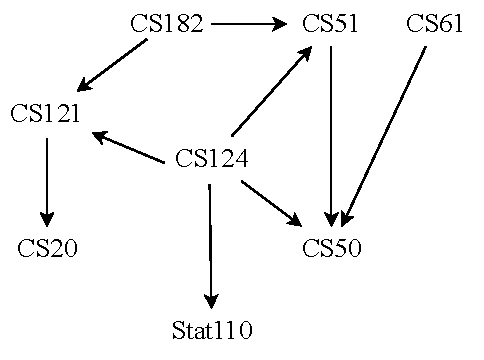
\includegraphics{graf.pdf}
            \caption{Graf av emner fra Figure 13.9}
        \end{figure*}
        \item Grafen er en DAG fordi ikke finnes noen sykler. Det gir ikke menning for en slik graf å ha sykler fordi da vil et emne kunne ende opp med å kreve seg selv som en forkunnskap, noe som ikke gir menning.
        \item Minste antall semester blir 3, fordelingen er:
        \begin{enumerate}
            \item [1.]semester: CS20, CS50, Stat110
            \item [2.]semester: CS51, CS61, CS121
            \item [3.]semester: CS124, CS182
        \end{enumerate}
    \end{enumerate}\newpage
    \item [\boxed{3}] For hvert hjørne \(v_i\), hvor \(i \in \mathbb{N}\), la \(x_i\) være ut-graden til \(v_i\), og \(y_i\) være inn-graden til \(v_i\).
    Dette gir 
    \[\sum^n_{i=1}(x^2_i - y^2_i) = \sum^n_{i=1}(x_i + y_i)(x_i - y_i)\]
    Fordi grafen er komplett, så er \(x_i + y_i\) konstant, nærmere bestemt \(n - 1\).
    \[\sum^n_{i=1}(x^2_i - y^2_i) = (n - 1) \sum^n_{i=1}(x_i - y_i)\]
    Dette gir at \[\sum^n_{i=1}(x_i - y_i) = 0 \quad\square\]
    \item [\boxed{4}] Diameteren til grafen er 3 (eks. B-A-E-D), den lengste syklen er 6 (eks. B-A-C-D-E-F-B).
    \item [\boxed{5}] \text{ }
    \begin{figure*}[h!]
        \centering
        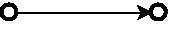
\includegraphics{graf2.pdf}
        \caption{En \emph{connected} graf som blir \emph{disconnected} ved å fjerne en kant}
    \end{figure*}
    \item [\boxed{6}] \(A-B-F-G-A-E-F-C-D-E-C-A\)
    \item [\boxed{7}]
    \begin{enumerate}
        \item \(b - e - f - e - d\)
        \item \(b - e - f - g - e - d\)
        \item \(b - e - d\)
        \item \(b - e - d - e - b\)
        \item \(b - e - f - g - e - d - c - b\)
        \item \(b - e - c - b\)
    \end{enumerate}

\end{enumerate}

% \printbibliography[heading=bibintoc] % LAGER BIBLIOGRAFI
\end{document}
